\section{Results}

Across all the censuses and traps/subplots, the data contained 666 species of tree, 26 species of small-mammal and 58 families of beetle. Output from the PCAs performed on each taxa separately but including all subplots/traps and census indicated that the first 3 components explained 28.89\%, 5.65\%, 4.44\% (cumulative 38.98\%) for trees, 26.44\%, 24.03\%, 11.34\% (cumulative 61.81\%) for mammals and 88.33\%, 7.59\%, 1.87\% (cumulative 97.79\%) for beetles.


\subsection{Comparison of Hypervolumes}

Hypervolumes were constructed for all plots and census and each census step within plots was compared. Figure \ref{fig:1} shows an example of a stable plot and a comparatively unstable plot. 

\begin{figure}[H]
	\centering
	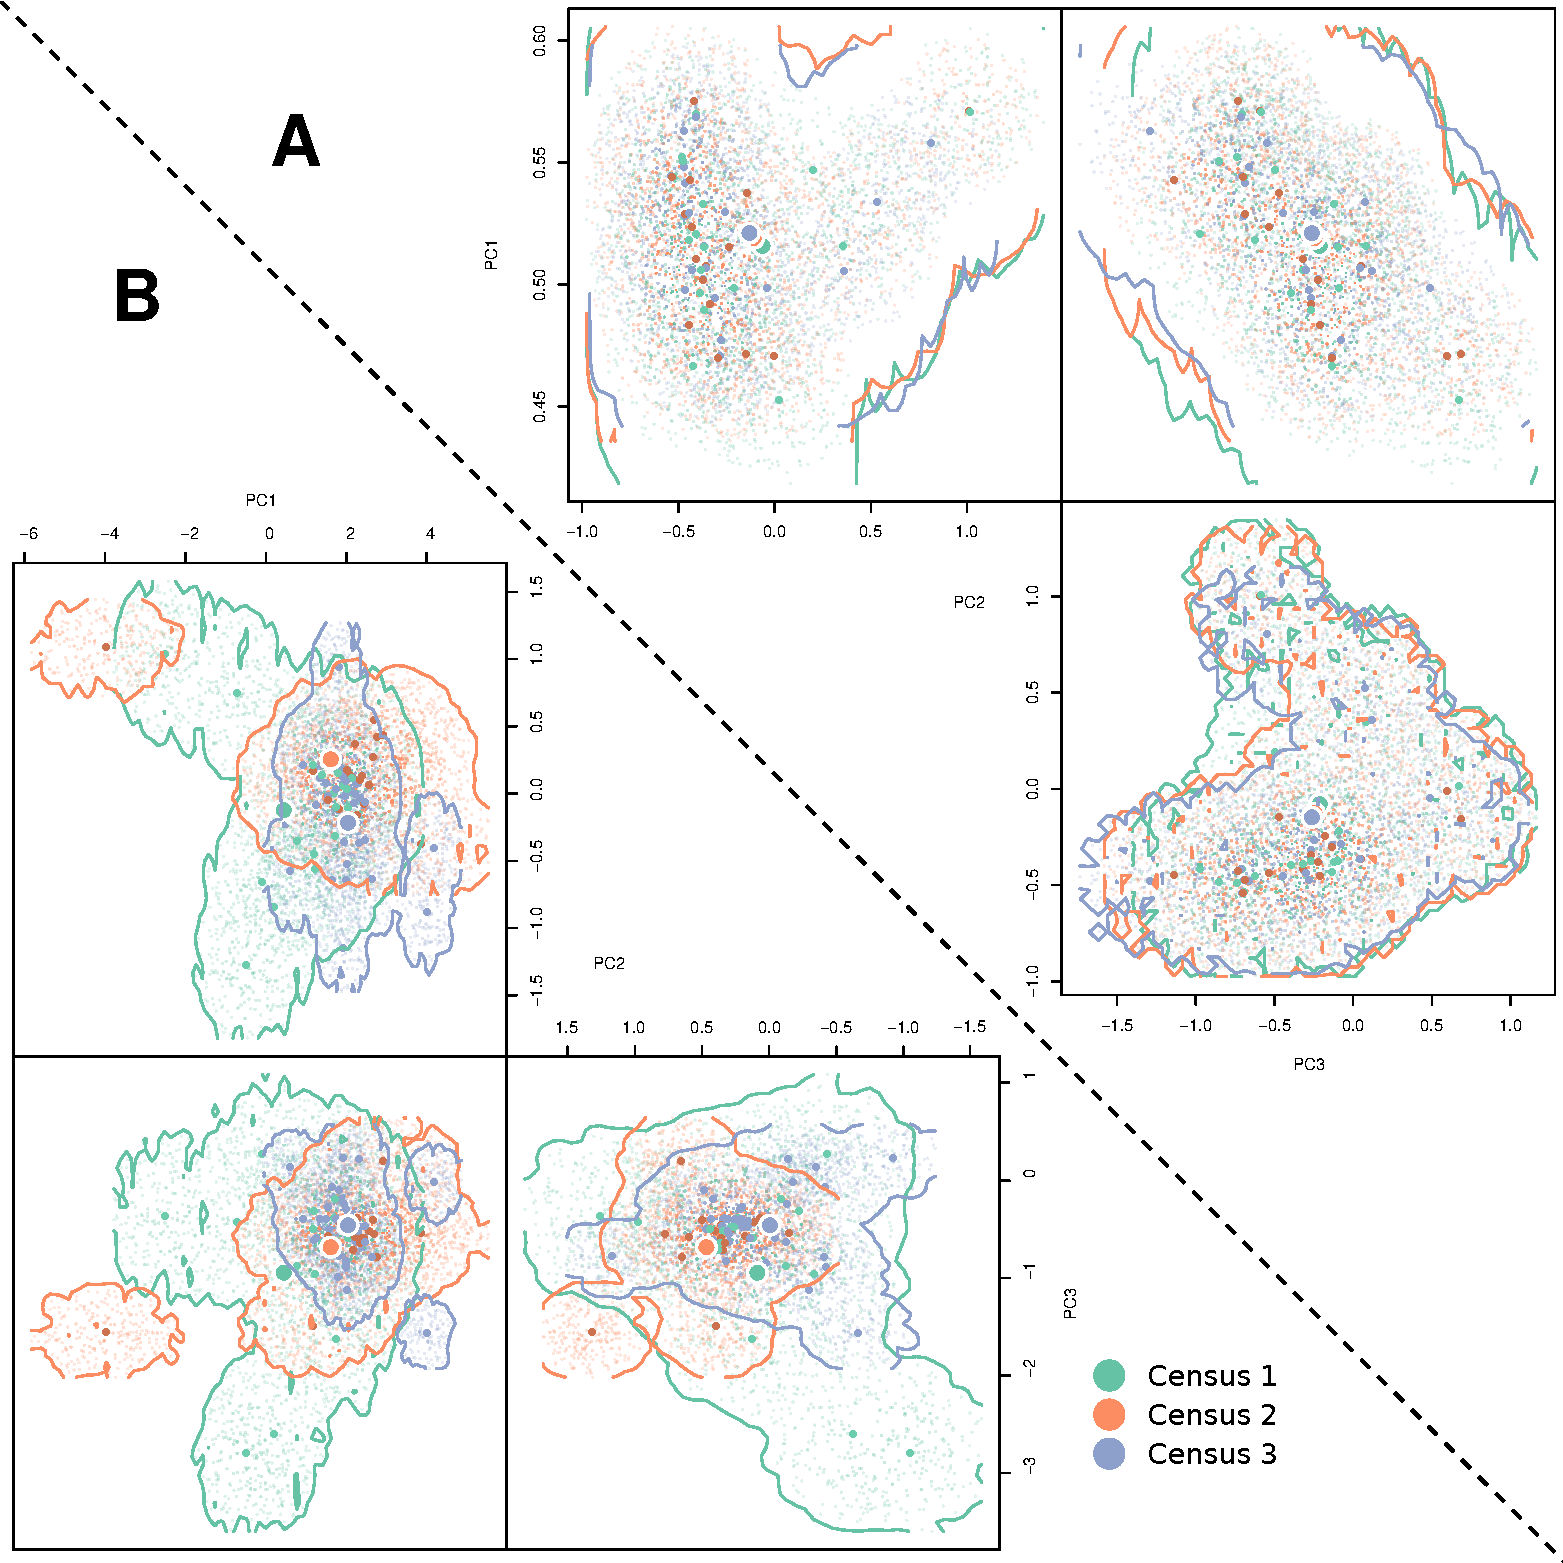
\includegraphics[width=\textwidth]{figures/figure1.pdf}
	\caption{\hl{here is my caption}}
	\label{fig:1}
\end{figure}	


\subsection{Effect of Taxa and Aboveground Biomass}

Trees were found to have significantly higher levels of hypervolume overlap when compared with mammals or beetles (figure \ref{fig:2} A \& B) \hl{Some Statistics}, while no difference was found in the other taxa. No effect of AGB was found to exist with level of hypervolume overlap in any of the taxa \hl{some statistics}.

\begin{figure}[H]
	\centering
	\includegraphics[width=\textwidth]{figures/figure2.pdf}
	\caption{\hl{here is my caption}}
	\label{fig:2}
\end{figure}


\subsection{Community Spatial Stability}

A similar pattern was found with this more traditional measure of stability, with trees having significantly higher levels of spatial stability than either of the other taxa \hl{some statistics}. With this measure there was an effect of AGB on the stability in trees (figure \ref{fig:2}D) however again this did not exist for the other taxa.


A significant correlation was found between this new measure of stability 'Hypervolume Overlap' and the calculated spatial stability for each plot (figure \ref{fig:3}). However this relationship did not exist when looking at individual taxa \hl{some statistics}.

\begin{figure}[H]
	\centering
	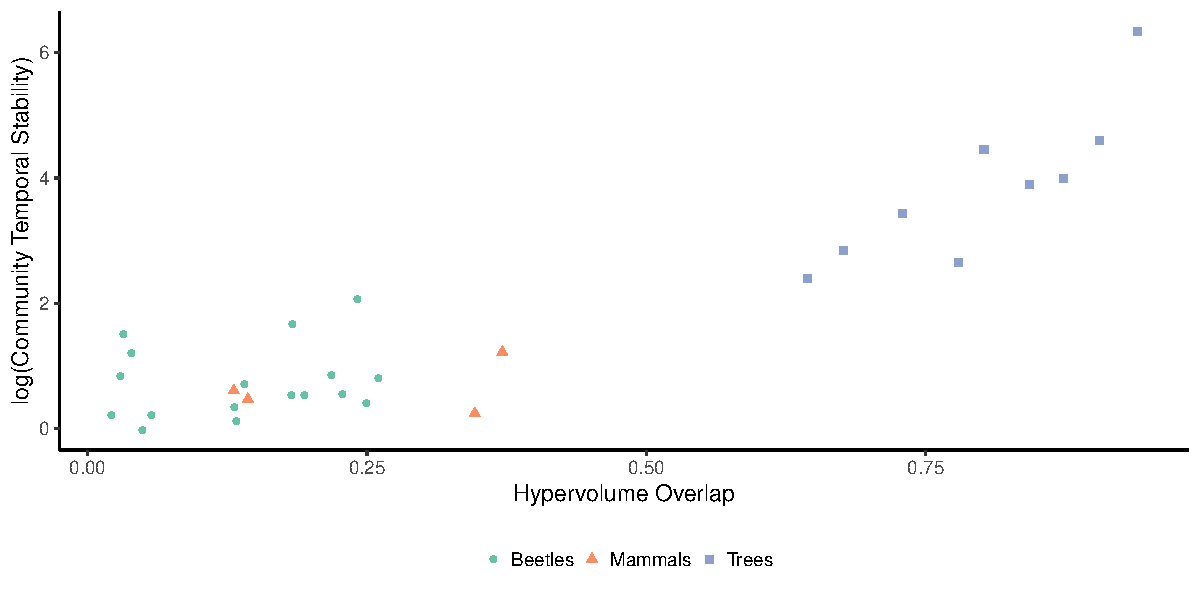
\includegraphics[width=\textwidth]{figures/figure3.pdf}
	\caption{\hl{here is my caption}}
	\label{fig:3}
\end{figure}
